\begin{frame}{PTVP tuyến tính}
    Phương trình vi phân tuyến tính là các phương trình chỉ bao gồm bậc nhất của các đạo hàm
    \begin{equation}
        \sum_{i=0}^n a_i x ^{(i)} = C.
        \label{eq:1.2_1}
    \end{equation}
    Khi chúng ta giải ra các nghiệm \((x_1, x_2,..., x_n)\) thoả mãn phương trình vi phân tuyến tính. Thì ta nói, nghiệm tổng quát là tổ hợp tuyến tính của các nghiệm
    \begin{equation}
        x_{tq} = A_1 x_1 + A_2 + ... + A_n x_n.
        \label{eq:1.2_2}
    \end{equation}
\end{frame}
\begin{frame}{Cộng dồn nghiệm}
\begin{center}
        \resizebox{0.6\linewidth}{!}{


\tikzset{every picture/.style={line width=0.75pt}} %set default line width to 0.75pt        

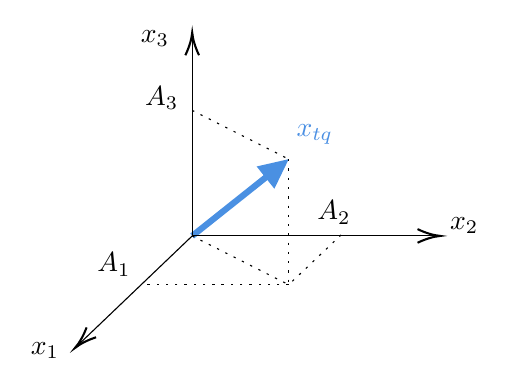
\begin{tikzpicture}[x=0.75pt,y=0.75pt,yscale=-1,xscale=1]
%uncomment if require: \path (0,15225); %set diagram left start at 0, and has height of 15225

%Straight Lines [id:da21513560769145257] 
\draw [color={rgb, 255:red, 74; green, 144; blue, 226 }  ,draw opacity=1 ][line width=2.25]    (204,5975) -- (246.59,5941.11) ;
\draw [shift={(250.5,5938)}, rotate = 141.49] [fill={rgb, 255:red, 74; green, 144; blue, 226 }  ,fill opacity=1 ][line width=0.08]  [draw opacity=0] (14.29,-6.86) -- (0,0) -- (14.29,6.86) -- cycle    ;
%Straight Lines [id:da8820661847854037] 
\draw    (204,5975) -- (321.5,5975) ;
\draw [shift={(323.5,5975)}, rotate = 180] [color={rgb, 255:red, 0; green, 0; blue, 0 }  ][line width=0.75]    (10.93,-3.29) .. controls (6.95,-1.4) and (3.31,-0.3) .. (0,0) .. controls (3.31,0.3) and (6.95,1.4) .. (10.93,3.29)   ;
%Straight Lines [id:da5315178017564863] 
\draw    (204,5975) -- (148.95,6027.62) ;
\draw [shift={(147.5,6029)}, rotate = 316.3] [color={rgb, 255:red, 0; green, 0; blue, 0 }  ][line width=0.75]    (10.93,-3.29) .. controls (6.95,-1.4) and (3.31,-0.3) .. (0,0) .. controls (3.31,0.3) and (6.95,1.4) .. (10.93,3.29)   ;
%Straight Lines [id:da14510782407127987] 
\draw    (204,5975) -- (204,5879) ;
\draw [shift={(204,5877)}, rotate = 90] [color={rgb, 255:red, 0; green, 0; blue, 0 }  ][line width=0.75]    (10.93,-3.29) .. controls (6.95,-1.4) and (3.31,-0.3) .. (0,0) .. controls (3.31,0.3) and (6.95,1.4) .. (10.93,3.29)   ;
%Straight Lines [id:da982507304256855] 
\draw  [dash pattern={on 0.84pt off 2.51pt}]  (250.5,5938) -- (250.5,5998.5) ;
%Straight Lines [id:da6681397441647374] 
\draw  [dash pattern={on 0.84pt off 2.51pt}]  (250.5,5998.5) -- (179.5,5998.5) ;
%Straight Lines [id:da7275191331520965] 
\draw  [dash pattern={on 0.84pt off 2.51pt}]  (204,5914.5) -- (250.5,5938) ;
%Straight Lines [id:da6882271778151009] 
\draw  [dash pattern={on 0.84pt off 2.51pt}]  (275.75,5974.5) -- (250.5,5998.5) ;
%Straight Lines [id:da4278104229055373] 
\draw  [dash pattern={on 0.84pt off 2.51pt}]  (204,5975) -- (250.5,5998.5) ;

% Text Node
\draw (253,5920) node [anchor=north west][inner sep=0.75pt]    {$\textcolor[rgb]{0.29,0.56,0.89}{x_{tq}}$};
% Text Node
\draw (125,6025) node [anchor=north west][inner sep=0.75pt]    {$x_{1}$};
% Text Node
\draw (327,5965) node [anchor=north west][inner sep=0.75pt]    {$x_{2}$};
% Text Node
\draw (178,5875) node [anchor=north west][inner sep=0.75pt]    {$x_{3}$};
% Text Node
\draw (157,5982) node [anchor=north west][inner sep=0.75pt]    {$A _{1}$};
% Text Node
\draw (263,5957) node [anchor=north west][inner sep=0.75pt]    {$A _{2}$};
% Text Node
\draw (180,5902) node [anchor=north west][inner sep=0.75pt]    {$A _{3}$};


\end{tikzpicture}}
\end{center}
\end{frame}